\section{Layout Evaluation}
The layout evaluation process aimed to assess the performance of the layout recognition system in accurately identifying and extracting different elements within the document layout.
\subsection{IOU Score}
The evaluation was conducted with all labels included, followed by a refinement process where caption and figure labels were filtered out. The rationale behind this refinement was to focus specifically on the recognition of text elements within the layout.

Upon evaluation, the system achieved an average IOU score of 0.66 when considering all labels. This score indicates the degree of overlap between the predicted bounding boxes and the ground truth bounding boxes for all elements in the layout. However, after filtering out caption and figure labels, the average IOU score increased to 0.81 This improvement demonstrates the effectiveness of the filtering process in refining the recognition accuracy for text components.

\subsection{F1-Score}
To further analyze the performance, F1 scores were calculated both with and without figure labels. The F1 score considers both precision and recall and provides an overall assessment of the system's performance. By comparing the F1 scores, we were able to observe the impact of including or excluding figure labels on the system's recognition performance. The results were plotted to visualize the difference in F1 scores between the two scenarios, shedding light on the effectiveness of focusing on text-only recognition.

\begin{figure}[H]
    \centering
    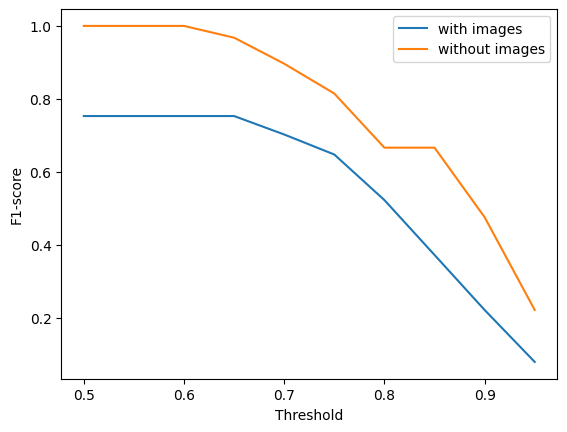
\includegraphics[width=0.6\textwidth]{Images/f1s.png}
    \caption{F1 scores across different thresholds}
    \label{fig:f1}
\end{figure}

The \textbf{Figure \ref{fig:f1}} of the F1 score plot across different thresholds provides a clear visualization of the performance comparison between the two scenarios: with and without images. 

As the threshold increases, the recognition system becomes more selective in identifying layout elements. 
When focusing solely on text recognition by excluding images, the F1 score consistently outperforms the scenario with images across all threshold values. This observation highlights the benefits of filtering out images and solely concentrating on text components in terms of achieving higher overall accuracy and performance.

Additionally, a precision-recall curve was plotted to provide a comprehensive understanding of the system's performance at various thresholds. 

\begin{figure}[H]
    \centering
    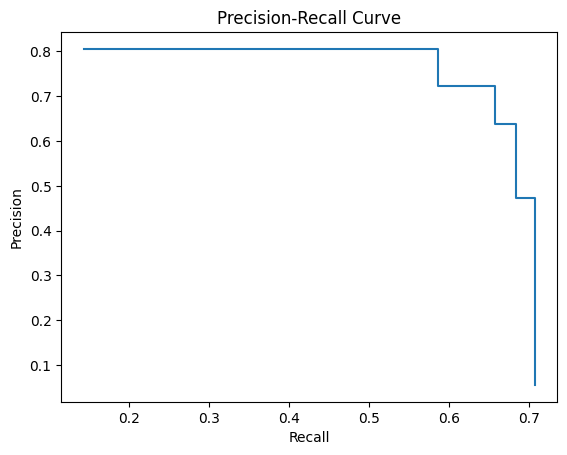
\includegraphics[width=0.6\textwidth]{Images/precision_recall.png}
    \caption{Precision-Recall curve across multiple thresholds}
    \label{fig:prec_rec}
\end{figure}

The curve in \textbf{Figure \ref{fig:prec_rec}} visually represents the trade-off between precision and recall, allowing for the identification of an optimal threshold based on the desired precision-recall trade-off. 
A higher precision indicates a lower number of false positives (layouts wrongly identified), while a higher recall indicates a lower number of false negatives (missed boxes).

At lower thresholds, where the system is more permissive in accepting predictions, both precision and recall tend to be higher. This indicates that more elements are correctly identified (higher recall), but there is also a higher chance of including false positives (lower precision).

Conversely, at higher thresholds, the system becomes more selective, resulting in lower recall as some correct elements may be missed. However, the precision increases since the accepted predictions are more likely to be correct.

\section{OCR results}
In the OCR results section, the focus was on evaluating the quality of the Optical Character Recognition (OCR) process applied to the scanned pages of the book. 

To ensure optimal OCR results, a high DPI (dots per inch) value of 300 was specified when loading the scanned pages using the lp.io.load\_pdf() method. This higher DPI value significantly improved the quality of the loaded pages, resulting in better OCR performance. It is worth noting that when the DPI value is lower, the scanned pages' loading quality tends to degrade, impacting the accuracy of the OCR process.

While various metrics, such as word-level or character-level accuracy, could have been employed to quantitatively evaluate the OCR results, it was determined that conducting such evaluations would be time-consuming and unnecessary. This decision was based on the understanding that the combination of good layout parsing and the high scanning quality of the book inherently implies good OCR accuracy. As a result, visual inspection was deemed sufficient to gain confidence in the overall quality of the OCR output.

Visual inspection involved manually reviewing the OCR results alongside the original scanned pages to ensure accurate and faithful transcription of the text. This qualitative evaluation method enabled the identification of any discrepancies or errors, providing a comprehensive understanding of the OCR performance. 

The evaluation of OCR results through visual inspection confirmed the high quality of the OCR output. The accurate layout parsing and the high scanning quality of the book contributed to the overall fidelity of the transcribed text.

\section{Database}
\subsection{Insertion Precision}
The evaluation of the database insertion process involved assessing the precision of the insertion for the main columns of the database. The precision was determined by examining the percentage of non-NaN (not inserted correctly) values in each column. 

The evaluation results are as follows:

\begin{table}[H]
\centering
\begin{tabular}{|>{\centering\arraybackslash}p{4cm}|>{\centering\arraybackslash}p{3cm}|}
\hline
\textbf{Column} & \textbf{Precision} \\ \hline
Name & 1.0 \\ \hline
Date\_id & 0.84375 \\ \hline
Type & 0.859375 \\ \hline
Modern\_name & 0.859375 \\ \hline
Hist\_id & 0.90625 \\ \hline
Arch\_id & 0.828125 \\ \hline
\end{tabular}
\caption{Database Insertion Evaluation}
\label{tab:database-evaluation}
\end{table}

It is important to consider that the presence of missing values in these columns is not solely attributable to the database insertion process. The missing values may also stem from earlier stages of the workflow, such as layout recognition and OCR. Therefore, it is crucial to acknowledge that the precision results are influenced by the quality and accuracy of the data obtained from these preceding steps.

The database insertion evaluation provides insights into the precision of inserting data into the main columns of the database. While some columns exhibit higher precision, others have a relatively lower precision due to missing values.

\subsection{Execution Time}
Moreover, an evaluation was conducted to assess the execution time of several sample queries. These queries were designed to retrieve specific information from the database and provide insights into its performance. The purpose of this evaluation was to analyze the efficiency and responsiveness of the database system when executing different types of queries.

The sample queries included:

\begin{itemize}
    \item Query 1:  \textit{"SELECT * FROM building WHERE name = '{}'".format(name)}\\
    Retrieving all columns from the "building" table based on a randomly selected building name.
    \item Query 2: \textit{"SELECT * FROM building"}\\
    Retrieving all columns from the "building" table.
    \item Query 3: \textit{"SELECT name, modern\_name FROM building"}\\
    Retrieving only the "name" and "modern\_name" columns from the "building" table.
    \item Query 4: \textit{"SELECT COUNT(*) FROM date"}\\
    Counting the total number of records in the "date" table.
    \item Query 5: \textit{"SELECT COUNT(DISTINCT subtitles) FROM architecture"}\\
    Counting the number of distinct values in the "subtitles" column of the "architecture" table.
    \item Query 6: \textit{"SELECT * FROM building JOIN date ON building.date\_id = date.id"}\\
    Performing a join operation between the "building" and "date" tables, retrieving all columns.
\end{itemize}

The execution times of these queries were measured and the results were plotted in a histogram, as shown below:

\begin{figure}[H]
\centering
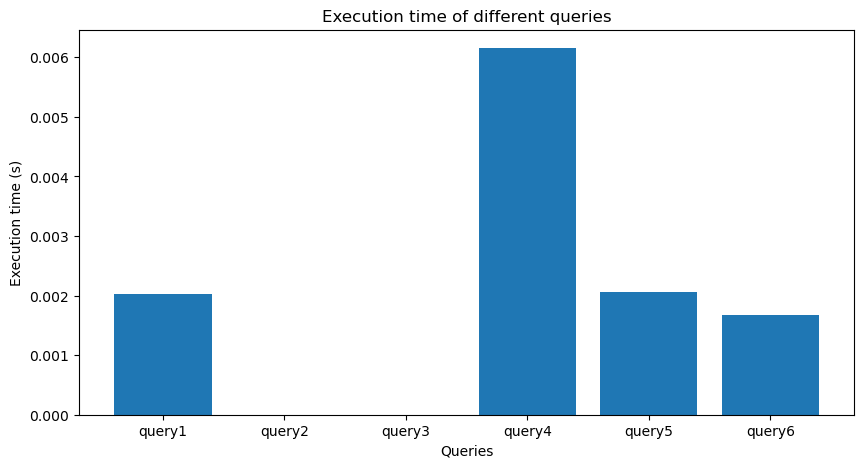
\includegraphics[width=0.8\textwidth]{Images/queries.png}
\caption{Execution Time of Sample Queries}
\label{fig:queries}
\end{figure}

Analyzing the histogram in \textbf{Figure \ref{fig:queries}}, we observe that the majority of the queries are executed within a very short time, with execution times close to zero. This indicates that the database system is highly efficient in handling these specific queries, resulting in fast response times.

\section{Leaflet Map}

The final result of the project is a leaflet map of Jerusalem displaying the locations of Mamluk buildings. The map incorporates various interactive features to enhance user experience and exploration of the architectural heritage.

\subsubsection{Search Bar}

The leaflet map includes a search bar that enables users to search for a specific building by its name. This feature enhances the accessibility and convenience of locating a particular building within the map. Users can simply select the building's name in the search bar, and the map will automatically navigate to the corresponding location.

\begin{figure}[H]
\centering
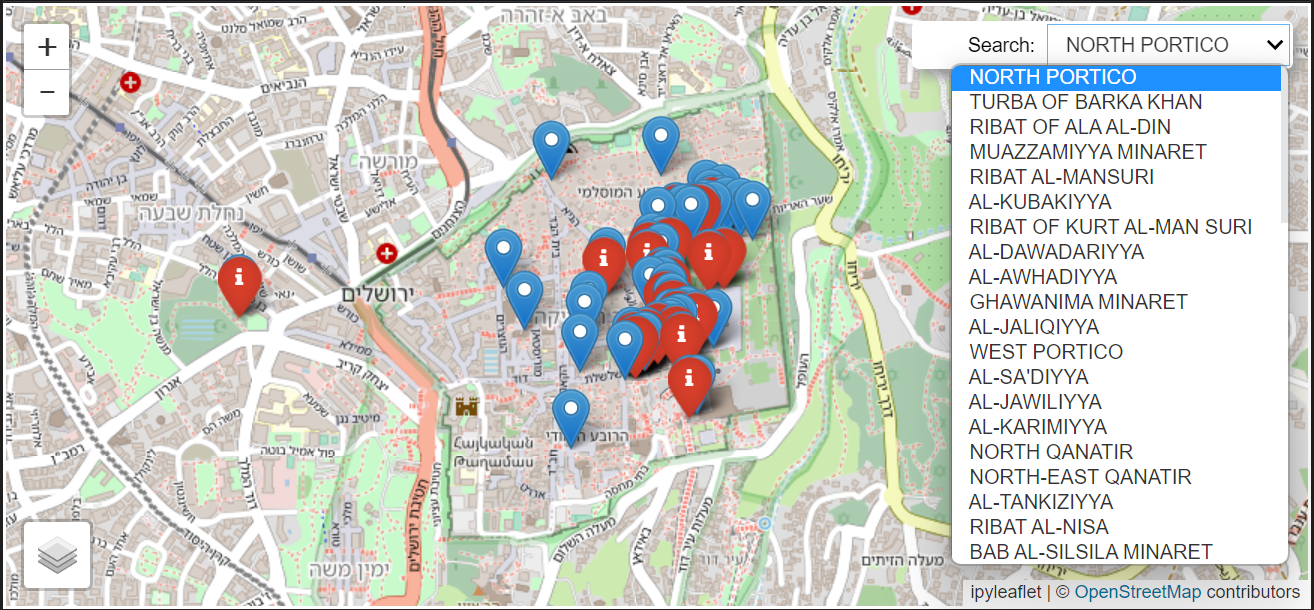
\includegraphics[width=0.8\textwidth]{Images/search_bar.png}
\caption{Search Bar}
\label{fig:search_bar}
\end{figure}

\subsubsection{Zoom In/Out}

The leaflet map provides users with the ability to zoom in and out, allowing for a closer look at specific areas or a broader view of the entire map.

\subsubsection{Layers}

The map incorporates a layers feature that provides two distinct map layers for better organization and visualization. The first layer (Figure \ref{fig:build_layer}) displays information about the Mamluk buildings, while the second layer (Figure \ref{fig:insc_layer}) focuses on inscriptions found within these buildings. \\[0.3cm]

\begin{figure}[H]
    \centering
    \begin{minipage}[c]{.5\linewidth}
        \centering
        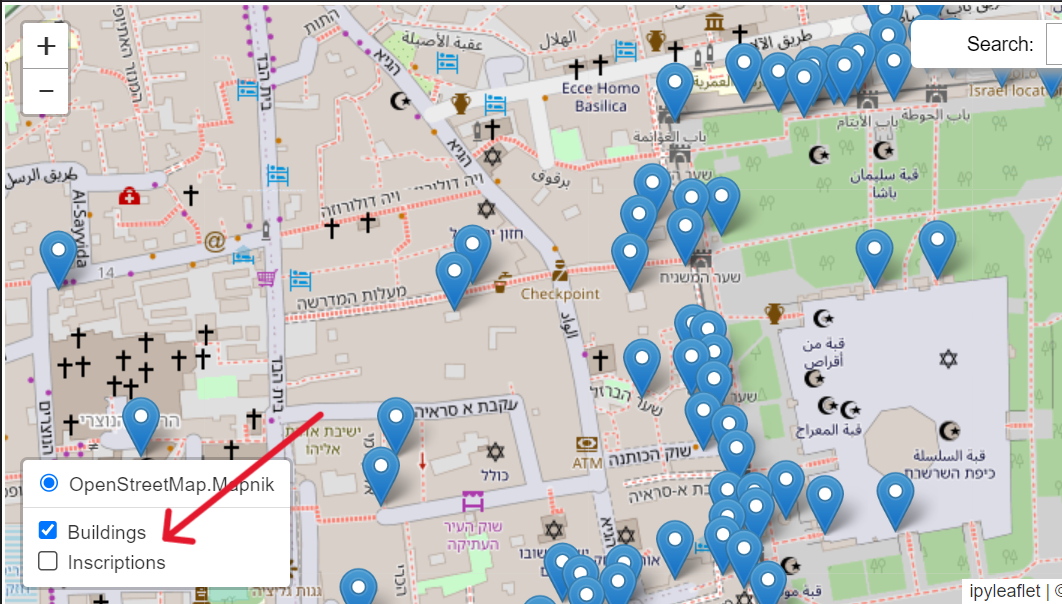
\includegraphics[width=0.9\textwidth]{Images/building_layer.png}
        \subcaption{Buildings Layer}
        \label{fig:build_layer}
    \end{minipage}\hfill
    \begin{minipage}[c]{.5\linewidth}
        \centering
        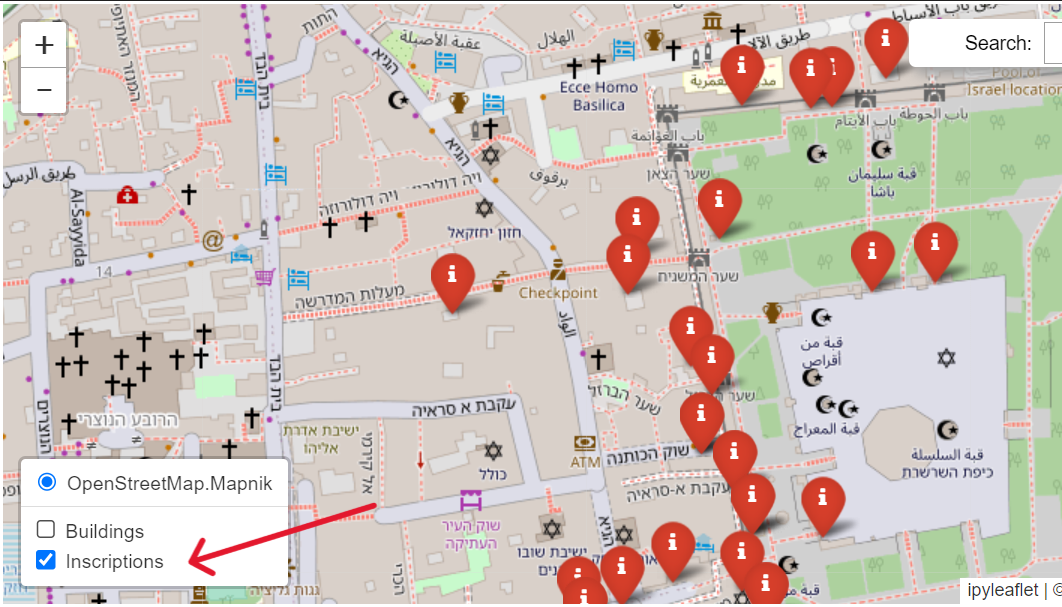
\includegraphics[width=0.9\textwidth]{Images/insc_layer.png}
        \subcaption{Inscriptions Layer}
        \label{fig:insc_layer}
    \end{minipage}
    \caption{Layers Feature}
    \label{fig:layers}
\end{figure}

\subsubsection{Building Marker Popups}

Each building marker on the map includes a popup or side pane that provides detailed information about the selected building. The popup is divided into four sections: General, Date, History, and Architecture.

\begin{figure}[H]
    \centering
    \begin{minipage}[c]{.5\linewidth}
        \centering
        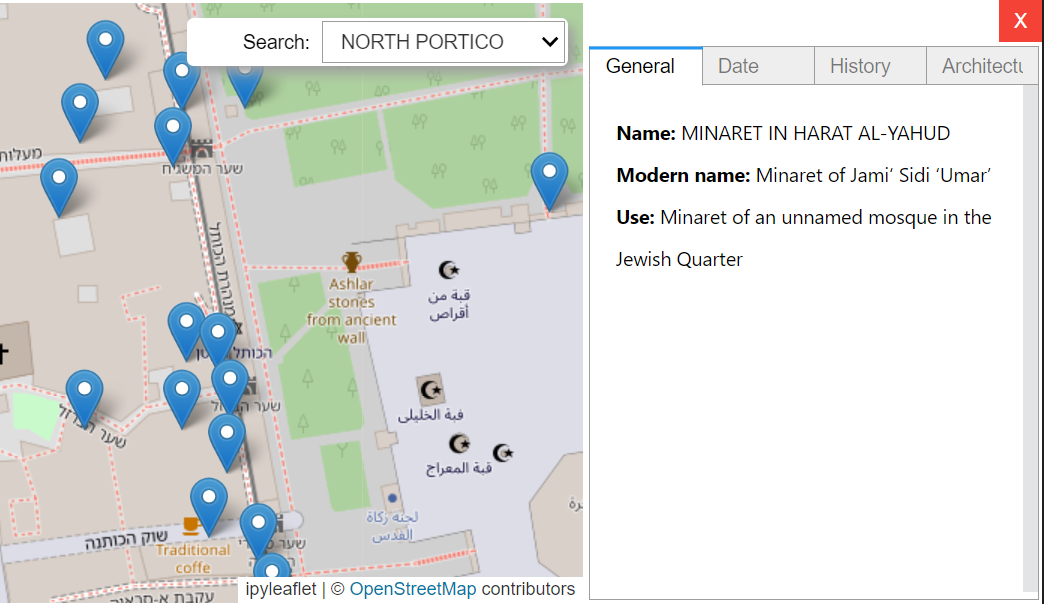
\includegraphics[width=0.9\textwidth]{Images/general.png}
        \subcaption{General Information}
        \label{fig:general}
    \end{minipage}\hfill
    \begin{minipage}[c]{.5\linewidth}
        \centering
        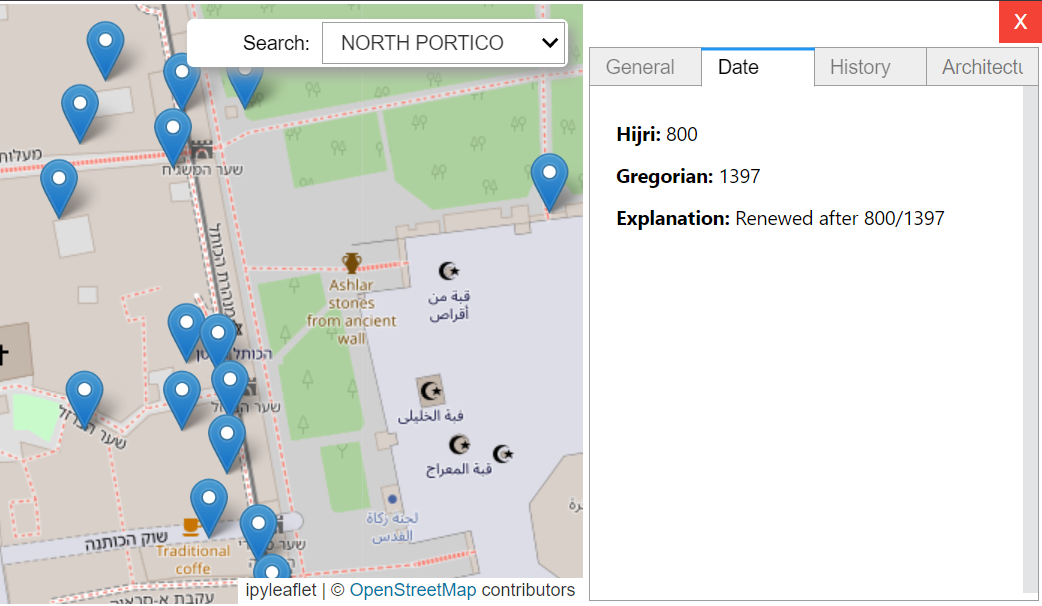
\includegraphics[width=0.9\textwidth]{Images/date.png}
        \subcaption{Date}
        \label{fig:date}
    \end{minipage}\\[0.3cm]
    \begin{minipage}[c]{.5\linewidth}
        \centering
        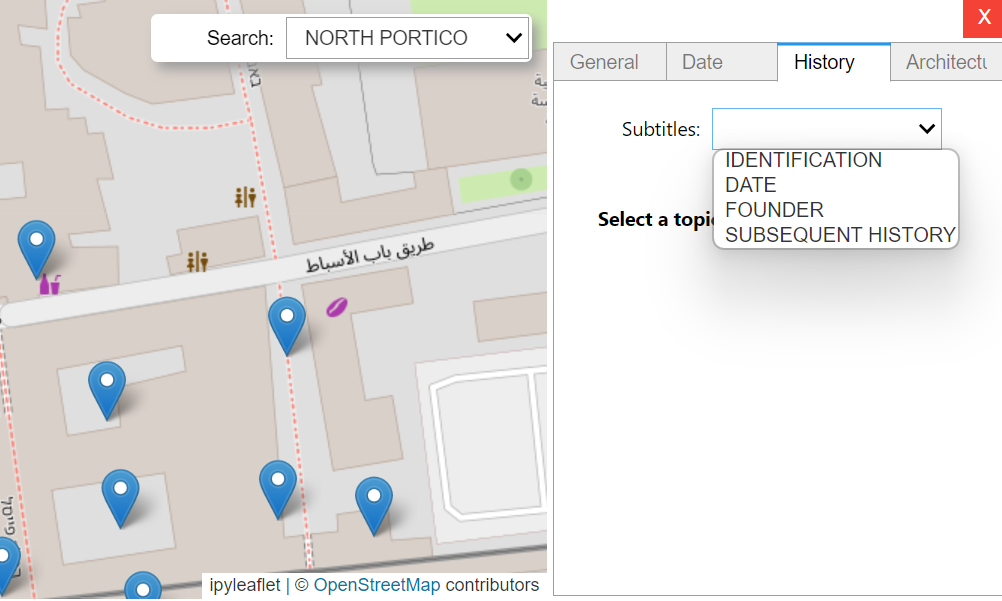
\includegraphics[width=0.9\textwidth]{Images/history.png}
        \subcaption{History}
        \label{fig:hist}
    \end{minipage}\hfill
    \begin{minipage}[c]{.5\linewidth}
        \centering
        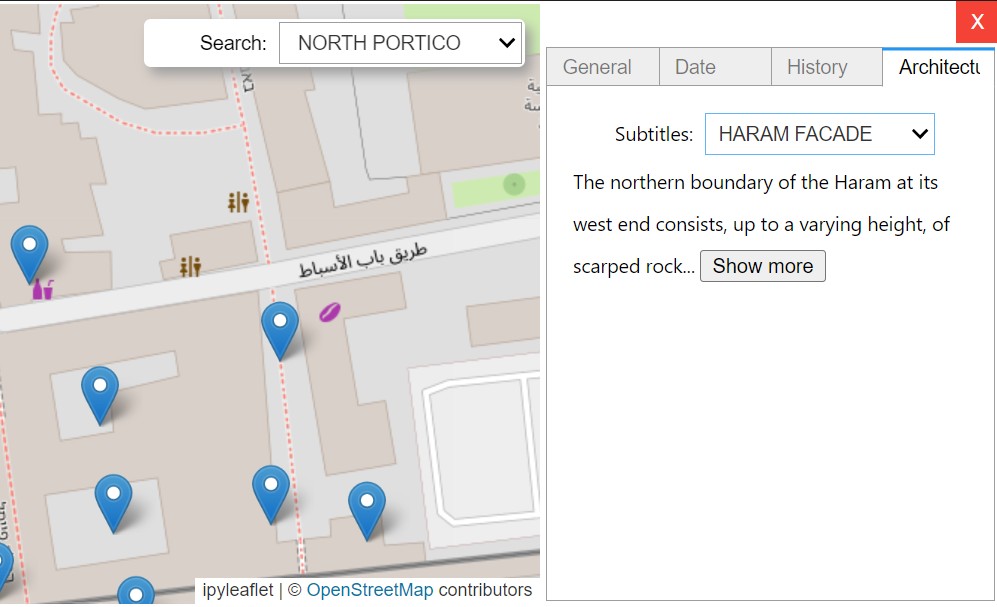
\includegraphics[width=0.9\textwidth]{Images/arch.png}
        \subcaption{Architecture}
        \label{fig:arch}
    \end{minipage}
    \caption{Buildings Popup}
    \label{fig:layers}
\end{figure}

\textbf{General}: This section (Figure \ref{fig:general}) presents key information about the building, including its name, modern name (if applicable), and use or purpose.

\textbf{Date}: The Date section (Figure \ref{fig:date}) includes the building's historical dates in both the Hijri (Islamic calendar) and Gregorian calendars. Additionally, an explanation of the date is provided to offer further context.

\textbf{History}: In the History section (Figure \ref{fig:hist}), users can access a dropdown menu of subtitles associated with the building. When a subtitle is selected from the dropdown, the corresponding content from the book article is displayed, providing insights into the building's historical significance.

\textbf{Architecture}: Similar to the History section (Figure \ref{fig:arch}), the Architecture section allows users to explore specific architectural aspects of the building by selecting different subtitles from the dropdown menu.

These interactive building marker popups offer a comprehensive understanding of each Mamluk building's details, history, and architectural features.

\subsubsection{Inscription Popup}

In addition to the building marker popups, the leaflet map includes a special feature for inscriptions. When a building marker on the map is clicked within the inscription layer, a side pane or popup displays all the inscriptions cited in the book specifically related to that building.

\begin{figure}[H]
\centering
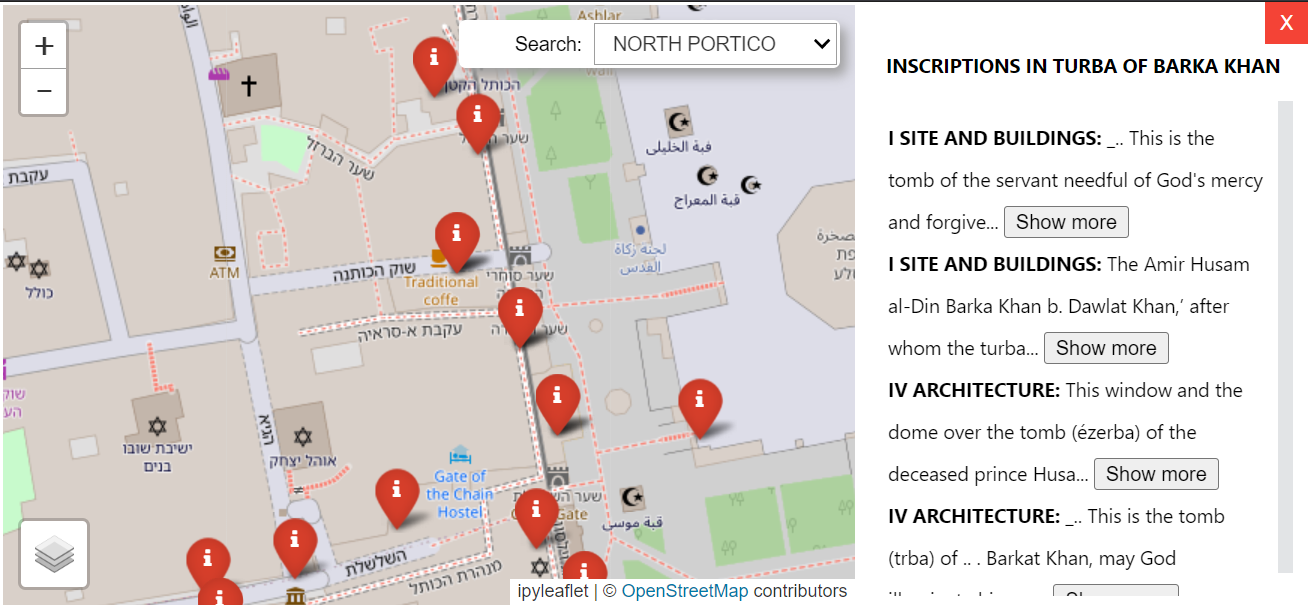
\includegraphics[width=0.8\textwidth]{Images/insc_popup.png}
\caption{Inscription Popup}
\label{fig:inscription_popup}
\end{figure}

The Inscription Popup in \textbf{Figure \ref{fig:inscription_popup}} provides users with a comprehensive view of the inscriptions found within the selected Mamluk building. Users can explore the textual content, calligraphy, and other details of these inscriptions, contributing to a deeper understanding of the historical and cultural significance associated with each building.

The Leaflet map, along with its interactive features and informative marker popups, serves as an engaging platform for users to explore and learn about the Mamluk architectural and cultural heritage in Jerusalem.


